% Created by tikzDevice version 0.7.0 on 2014-04-27 13:00:35
% !TEX encoding = UTF-8 Unicode
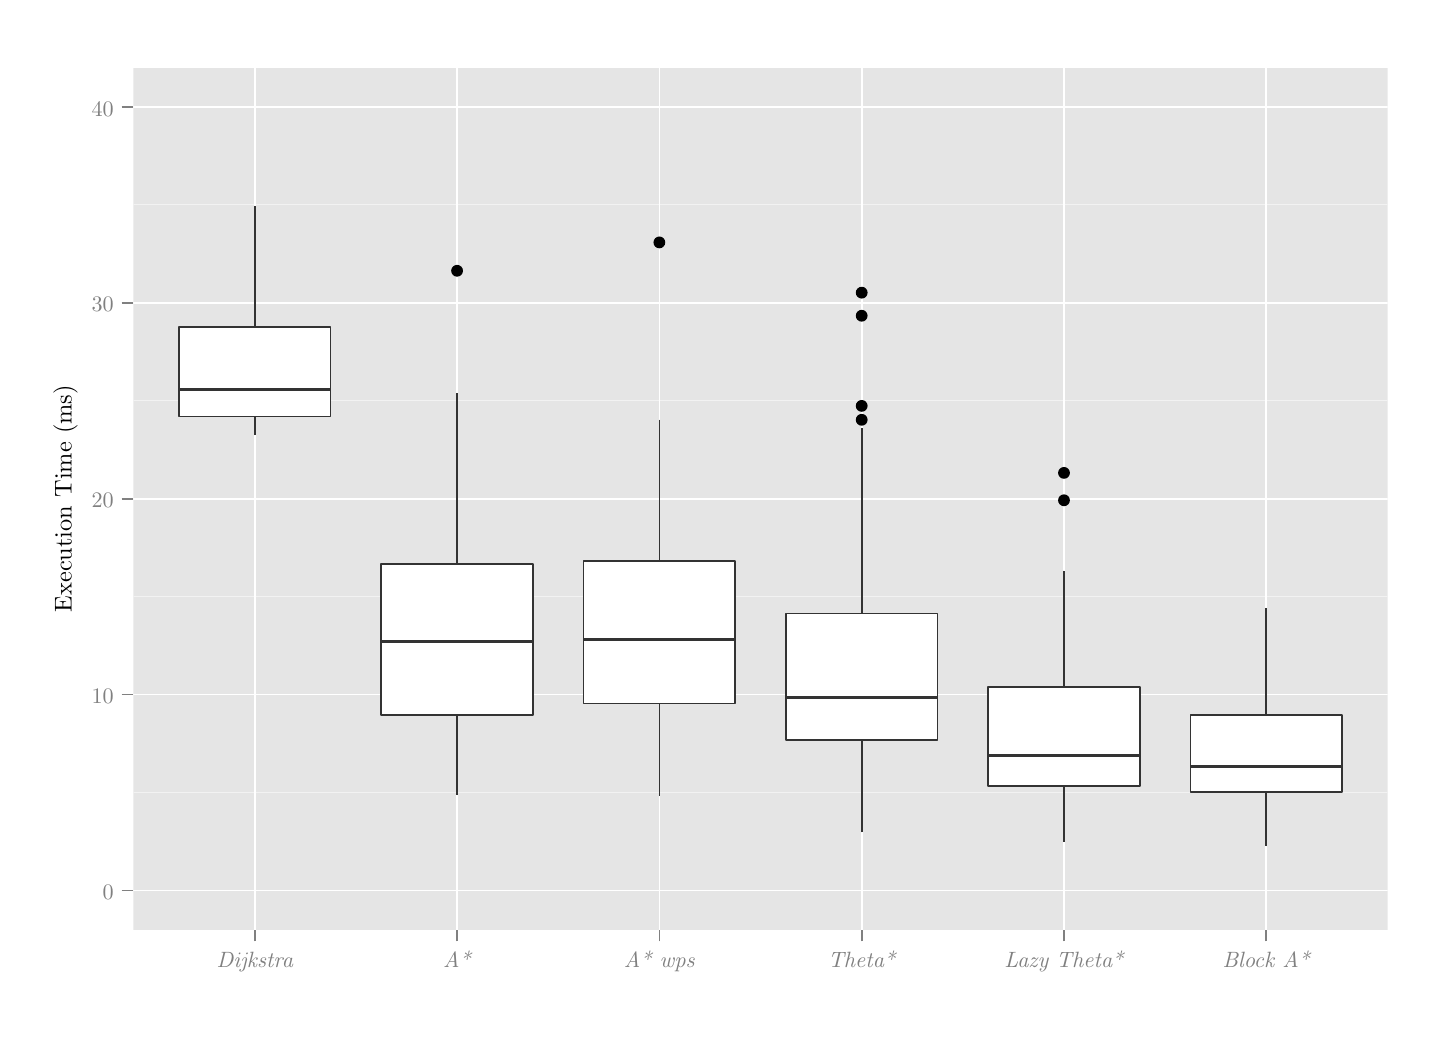
\begin{tikzpicture}[x=1pt,y=1pt]
\definecolor[named]{fillColor}{rgb}{1.00,1.00,1.00}
\path[use as bounding box,fill=fillColor,fill opacity=0.00] (0,0) rectangle (505.89,361.35);
\begin{scope}
\path[clip] (  0.00,  0.00) rectangle (505.89,361.35);
\definecolor[named]{drawColor}{rgb}{1.00,1.00,1.00}
\definecolor[named]{fillColor}{rgb}{1.00,1.00,1.00}

\path[draw=drawColor,line width= 0.6pt,line join=round,line cap=round,fill=fillColor] (  0.00, -0.00) rectangle (505.89,361.35);
\end{scope}
\begin{scope}
\path[clip] ( 38.20, 35.41) rectangle (491.44,346.90);
\definecolor[named]{fillColor}{rgb}{0.90,0.90,0.90}

\path[fill=fillColor] ( 38.20, 35.41) rectangle (491.44,346.90);
\definecolor[named]{drawColor}{rgb}{0.95,0.95,0.95}

\path[draw=drawColor,line width= 0.3pt,line join=round] ( 38.20, 84.97) --
	(491.44, 84.97);

\path[draw=drawColor,line width= 0.3pt,line join=round] ( 38.20,155.76) --
	(491.44,155.76);

\path[draw=drawColor,line width= 0.3pt,line join=round] ( 38.20,226.55) --
	(491.44,226.55);

\path[draw=drawColor,line width= 0.3pt,line join=round] ( 38.20,297.34) --
	(491.44,297.34);
\definecolor[named]{drawColor}{rgb}{1.00,1.00,1.00}

\path[draw=drawColor,line width= 0.6pt,line join=round] ( 38.20, 49.57) --
	(491.44, 49.57);

\path[draw=drawColor,line width= 0.6pt,line join=round] ( 38.20,120.36) --
	(491.44,120.36);

\path[draw=drawColor,line width= 0.6pt,line join=round] ( 38.20,191.15) --
	(491.44,191.15);

\path[draw=drawColor,line width= 0.6pt,line join=round] ( 38.20,261.95) --
	(491.44,261.95);

\path[draw=drawColor,line width= 0.6pt,line join=round] ( 38.20,332.74) --
	(491.44,332.74);

\path[draw=drawColor,line width= 0.6pt,line join=round] ( 82.06, 35.41) --
	( 82.06,346.90);

\path[draw=drawColor,line width= 0.6pt,line join=round] (155.16, 35.41) --
	(155.16,346.90);

\path[draw=drawColor,line width= 0.6pt,line join=round] (228.26, 35.41) --
	(228.26,346.90);

\path[draw=drawColor,line width= 0.6pt,line join=round] (301.37, 35.41) --
	(301.37,346.90);

\path[draw=drawColor,line width= 0.6pt,line join=round] (374.47, 35.41) --
	(374.47,346.90);

\path[draw=drawColor,line width= 0.6pt,line join=round] (447.57, 35.41) --
	(447.57,346.90);
\definecolor[named]{drawColor}{rgb}{0.20,0.20,0.20}
\definecolor[named]{fillColor}{rgb}{0.20,0.20,0.20}

\path[draw=drawColor,line width= 0.6pt,line join=round,fill=fillColor] ( 82.06,253.22) -- ( 82.06,296.96);

\path[draw=drawColor,line width= 0.6pt,line join=round,fill=fillColor] ( 82.06,220.83) -- ( 82.06,214.09);
\definecolor[named]{fillColor}{rgb}{1.00,1.00,1.00}

\path[draw=drawColor,line width= 0.6pt,line join=round,line cap=round,fill=fillColor] ( 54.64,253.22) --
	( 54.64,220.83) --
	(109.47,220.83) --
	(109.47,253.22) --
	( 54.64,253.22) --
	cycle;
\definecolor[named]{fillColor}{rgb}{0.20,0.20,0.20}

\path[draw=drawColor,line width= 1.1pt,line join=round,fill=fillColor] ( 54.64,230.67) -- (109.47,230.67);
\definecolor[named]{fillColor}{rgb}{0.00,0.00,0.00}

\path[fill=fillColor] (155.16,273.50) circle (  2.13);
\definecolor[named]{fillColor}{rgb}{0.20,0.20,0.20}

\path[draw=drawColor,line width= 0.6pt,line join=round,fill=fillColor] (155.16,167.44) -- (155.16,229.20);

\path[draw=drawColor,line width= 0.6pt,line join=round,fill=fillColor] (155.16,113.10) -- (155.16, 84.00);
\definecolor[named]{fillColor}{rgb}{1.00,1.00,1.00}

\path[draw=drawColor,line width= 0.6pt,line join=round,line cap=round,fill=fillColor] (127.75,167.44) --
	(127.75,113.10) --
	(182.58,113.10) --
	(182.58,167.44) --
	(127.75,167.44) --
	cycle;
\definecolor[named]{fillColor}{rgb}{0.20,0.20,0.20}

\path[draw=drawColor,line width= 1.1pt,line join=round,fill=fillColor] (127.75,139.54) -- (182.58,139.54);
\definecolor[named]{fillColor}{rgb}{0.00,0.00,0.00}

\path[fill=fillColor] (228.26,283.76) circle (  2.13);
\definecolor[named]{fillColor}{rgb}{0.20,0.20,0.20}

\path[draw=drawColor,line width= 0.6pt,line join=round,fill=fillColor] (228.26,168.67) -- (228.26,219.76);

\path[draw=drawColor,line width= 0.6pt,line join=round,fill=fillColor] (228.26,117.08) -- (228.26, 83.74);
\definecolor[named]{fillColor}{rgb}{1.00,1.00,1.00}

\path[draw=drawColor,line width= 0.6pt,line join=round,line cap=round,fill=fillColor] (200.85,168.67) --
	(200.85,117.08) --
	(255.68,117.08) --
	(255.68,168.67) --
	(200.85,168.67) --
	cycle;
\definecolor[named]{fillColor}{rgb}{0.20,0.20,0.20}

\path[draw=drawColor,line width= 1.1pt,line join=round,fill=fillColor] (200.85,140.28) -- (255.68,140.28);
\definecolor[named]{fillColor}{rgb}{0.00,0.00,0.00}

\path[fill=fillColor] (301.37,257.25) circle (  2.13);

\path[fill=fillColor] (301.37,219.65) circle (  2.13);

\path[fill=fillColor] (301.37,224.68) circle (  2.13);

\path[fill=fillColor] (301.37,265.59) circle (  2.13);
\definecolor[named]{fillColor}{rgb}{0.20,0.20,0.20}

\path[draw=drawColor,line width= 0.6pt,line join=round,fill=fillColor] (301.37,149.68) -- (301.37,216.77);

\path[draw=drawColor,line width= 0.6pt,line join=round,fill=fillColor] (301.37,104.01) -- (301.37, 70.59);
\definecolor[named]{fillColor}{rgb}{1.00,1.00,1.00}

\path[draw=drawColor,line width= 0.6pt,line join=round,line cap=round,fill=fillColor] (273.95,149.68) --
	(273.95,104.01) --
	(328.78,104.01) --
	(328.78,149.68) --
	(273.95,149.68) --
	cycle;
\definecolor[named]{fillColor}{rgb}{0.20,0.20,0.20}

\path[draw=drawColor,line width= 1.1pt,line join=round,fill=fillColor] (273.95,119.45) -- (328.78,119.45);
\definecolor[named]{fillColor}{rgb}{0.00,0.00,0.00}

\path[fill=fillColor] (374.47,190.57) circle (  2.13);

\path[fill=fillColor] (374.47,200.47) circle (  2.13);
\definecolor[named]{fillColor}{rgb}{0.20,0.20,0.20}

\path[draw=drawColor,line width= 0.6pt,line join=round,fill=fillColor] (374.47,123.21) -- (374.47,165.14);

\path[draw=drawColor,line width= 0.6pt,line join=round,fill=fillColor] (374.47, 87.26) -- (374.47, 67.13);
\definecolor[named]{fillColor}{rgb}{1.00,1.00,1.00}

\path[draw=drawColor,line width= 0.6pt,line join=round,line cap=round,fill=fillColor] (347.06,123.21) --
	(347.06, 87.26) --
	(401.88, 87.26) --
	(401.88,123.21) --
	(347.06,123.21) --
	cycle;
\definecolor[named]{fillColor}{rgb}{0.20,0.20,0.20}

\path[draw=drawColor,line width= 1.1pt,line join=round,fill=fillColor] (347.06, 98.46) -- (401.88, 98.46);

\path[draw=drawColor,line width= 0.6pt,line join=round,fill=fillColor] (447.57,113.05) -- (447.57,151.48);

\path[draw=drawColor,line width= 0.6pt,line join=round,fill=fillColor] (447.57, 85.11) -- (447.57, 65.62);
\definecolor[named]{fillColor}{rgb}{1.00,1.00,1.00}

\path[draw=drawColor,line width= 0.6pt,line join=round,line cap=round,fill=fillColor] (420.16,113.05) --
	(420.16, 85.11) --
	(474.99, 85.11) --
	(474.99,113.05) --
	(420.16,113.05) --
	cycle;
\definecolor[named]{fillColor}{rgb}{0.20,0.20,0.20}

\path[draw=drawColor,line width= 1.1pt,line join=round,fill=fillColor] (420.16, 94.52) -- (474.99, 94.52);
\end{scope}
\begin{scope}
\path[clip] (  0.00,  0.00) rectangle (505.89,361.35);
\definecolor[named]{drawColor}{rgb}{0.50,0.50,0.50}

\node[text=drawColor,anchor=base east,inner sep=0pt, outer sep=0pt, scale=  0.80] at ( 31.08, 46.26) {0};

\node[text=drawColor,anchor=base east,inner sep=0pt, outer sep=0pt, scale=  0.80] at ( 31.08,117.06) {10};

\node[text=drawColor,anchor=base east,inner sep=0pt, outer sep=0pt, scale=  0.80] at ( 31.08,187.85) {20};

\node[text=drawColor,anchor=base east,inner sep=0pt, outer sep=0pt, scale=  0.80] at ( 31.08,258.64) {30};

\node[text=drawColor,anchor=base east,inner sep=0pt, outer sep=0pt, scale=  0.80] at ( 31.08,329.43) {40};
\end{scope}
\begin{scope}
\path[clip] (  0.00,  0.00) rectangle (505.89,361.35);
\definecolor[named]{drawColor}{rgb}{0.50,0.50,0.50}

\path[draw=drawColor,line width= 0.6pt,line join=round] ( 33.93, 49.57) --
	( 38.20, 49.57);

\path[draw=drawColor,line width= 0.6pt,line join=round] ( 33.93,120.36) --
	( 38.20,120.36);

\path[draw=drawColor,line width= 0.6pt,line join=round] ( 33.93,191.15) --
	( 38.20,191.15);

\path[draw=drawColor,line width= 0.6pt,line join=round] ( 33.93,261.95) --
	( 38.20,261.95);

\path[draw=drawColor,line width= 0.6pt,line join=round] ( 33.93,332.74) --
	( 38.20,332.74);
\end{scope}
\begin{scope}
\path[clip] (  0.00,  0.00) rectangle (505.89,361.35);
\definecolor[named]{drawColor}{rgb}{0.50,0.50,0.50}

\path[draw=drawColor,line width= 0.6pt,line join=round] ( 82.06, 31.14) --
	( 82.06, 35.41);

\path[draw=drawColor,line width= 0.6pt,line join=round] (155.16, 31.14) --
	(155.16, 35.41);

\path[draw=drawColor,line width= 0.6pt,line join=round] (228.26, 31.14) --
	(228.26, 35.41);

\path[draw=drawColor,line width= 0.6pt,line join=round] (301.37, 31.14) --
	(301.37, 35.41);

\path[draw=drawColor,line width= 0.6pt,line join=round] (374.47, 31.14) --
	(374.47, 35.41);

\path[draw=drawColor,line width= 0.6pt,line join=round] (447.57, 31.14) --
	(447.57, 35.41);
\end{scope}
\begin{scope}
\path[clip] (  0.00,  0.00) rectangle (505.89,361.35);
\definecolor[named]{drawColor}{rgb}{0.50,0.50,0.50}

\node[text=drawColor,anchor=base,inner sep=0pt, outer sep=0pt, scale=  0.80] at ( 82.06, 21.69) {{\em Dijkstra}};

\node[text=drawColor,anchor=base,inner sep=0pt, outer sep=0pt, scale=  0.80] at (155.16, 21.69) {{\em A*}};

\node[text=drawColor,anchor=base,inner sep=0pt, outer sep=0pt, scale=  0.80] at (228.26, 21.69) {{\em A* wps}};

\node[text=drawColor,anchor=base,inner sep=0pt, outer sep=0pt, scale=  0.80] at (301.37, 21.69) {{\em Theta*}};

\node[text=drawColor,anchor=base,inner sep=0pt, outer sep=0pt, scale=  0.80] at (374.47, 21.69) {{\em Lazy Theta*}};

\node[text=drawColor,anchor=base,inner sep=0pt, outer sep=0pt, scale=  0.80] at (447.57, 21.69) {{\em Block A*}};
\end{scope}
\begin{scope}
\path[clip] (  0.00,  0.00) rectangle (505.89,361.35);
\definecolor[named]{drawColor}{rgb}{0.00,0.00,0.00}

\node[text=drawColor,rotate= 90.00,anchor=base,inner sep=0pt, outer sep=0pt, scale=  0.88] at ( 15.90,191.15) {Execution Time (ms)};
\end{scope}
\end{tikzpicture}
